\documentclass{mcmthesis}
\usepackage{ctex}
\mcmsetup{tstyle=\color{red}\bfseries,%修改题号，队号的颜色和加粗显示，黑色可以修改为 black
        tcn = 2600043, problem = F, %修改队号，参赛题号
        sheet = true, titleinsheet = false, keywordsinsheet = true,%修改sheet显示信息
        titlepage = false, abstract = true}



  %四款字体可以选择
  \usepackage{times}
  %\usepackage{newtxtext,newtxmath} %CTeX 无此字体，可用 txfonts 替代，请使用新版 TeXLive.
  %\usepackage{palatino}
  %\usepackage{txfonts}

%\usepackage{indentfirst}  %首行缩进，注释掉，首行就不再缩进。
\usepackage{lipsum}
\usepackage{etoolbox}
\usepackage{booktabs}
\usepackage{tabularx}   % optional (not used below)
\usepackage{arydshln}   % for dashed rules: \cdashline
\usepackage{caption}
\usepackage{float} 
\usepackage{booktabs} % 用于表格美观横线，必加
\title{To use generative AI or not to use it—that is the question!}



\date{\today}
\renewcommand{\contentsname}{\rmfamily Contents}
\pretocmd{\tableofcontents}{\begingroup\rmfamily}{}{}
\apptocmd{\tableofcontents}{\endgroup}{}{}

\begin{document}


\begin{abstract}
\par Use this template to begin writing the first page of your electronic report (Summary Sheet). This template defaults to a 12-point Times New Roman font. Submit your thesis as an Adobe PDF electronic file (e.g., 1111111.pdf), written in English, ensuring the font is clear and legible with a size no smaller than 12 points.

Do not include any identifying information such as school name, advisor's name, or team member names on this page or any other page.

Be sure to modify the control number and problem choice at the top.

When beginning formal writing, you may delete these instructions.

\textbf{Follow our social media @COMAPMath (Twitter) or COMAPCHINAOFFICIAL (Weibo) for the latest competition updates.}

\begin{keywords}
Keyword1; Keyword2
\end{keywords}
\end{abstract}



\maketitle
%% Generate the Table of Contents, if it's needed.
\tableofcontents
\newpage
%%
%% Generate the Memorandum, if it's needed.
%% \memoto{\LaTeX{}studio}
%% \memofrom{Liam Huang}
%% \memosubject{Happy \TeX{}ing!}
%% \memodate{\today}
%% \memologo{\LARGE I'm pretending to be a LOGO!}
%% \begin{memo}[Memorandum]
%%   \lipsum[1-3]
%% \end{memo}
%%



%%----------------------------------------------------------------------------------
%%----------------------------------------------------------------------------------
\section{Introduction}
%%----------------------------------------------------------------------------------

\subsection{Problem Background}
\noindent In recent years, generative artificial intelligence has become deeply embedded in learning and work processes, providing support in writing, programming, design, information retrieval, and content generation, while reshaping workflows across various job roles. Employer surveys indicate that demand for key professional skills will change significantly in the coming years, making bridging the AI skills gap a critical challenge for businesses. The impact of AI development on the future of careers and the resulting transformation of talent development models have drawn widespread attention.


\noindent Despite the widespread acceleration of AI diffusion across various fields, its impact on different occupations exhibits significant heterogeneity. While generative AI can support or partially complete numerous tasks in certain professions, others rely more heavily on on-site operations or interpersonal collaboration. Task-level estimates indicate that approximately one-quarter of the global workforce will experience varying degrees of impact. Common outcomes tend to be job restructuring and upskilling rather than direct job replacement. This projection creates an urgent imperative for education systems: curricula and assessment frameworks must be promptly adapted to equip students with the skills to leverage generative AI for capability enhancement while mitigating its negative consequences. Concurrently, the proliferation of generative AI imposes resource and environmental pressures. Model training and deployment consume substantial electricity, while hardware cooling increases water usage, impacting local water resources and ecosystems. Therefore, there is an urgent need to employ data-driven methods to identify representative key occupations under AI penetration, systematically predict their development trajectories, and use these insights to inform educational model optimization and policy decision-making.

\begin{figure}[ht!]
  \centering
  
\includegraphics[width=0.98\linewidth]{gen-AI_impact_evidence.png}
  \caption{Gen-AI Impact Evidence. These charts synthesize multiple datasets\cite{WEF2023,IEA2023,ILO2023,ITBrew,CensusBTOS} to illustrate the impact of Gen-AI on contemporary society and the environment.}
  \label{fig:Gen-AI Impact Evidence}
\end{figure}

\noindent Against this backdrop, this study connects labor-market shifts to educational decision-making through data-driven analysis. The study first analyzes task evolution and skill demands across occupations, then translates these findings into actionable adjustments for schools and specific training programs. These adjustments encompass curriculum content, practical training, assessment design, faculty allocation, and risk management measures such as usage protocols, attribution, and acknowledgments. Through multi-indicator evaluation and uncertainty analysis, the research aims to provide more robust recommendations and construct a reusable decision-making framework applicable to diverse training programs.





%%----------------------------------------------------------------------------------
\subsection{Problem Restatement}
\noindent\textbf{Problem 1:} Identify the most promising occupations for focused research across a wide range of professions, ensuring they represent key types of change and ultimately cover one occupation each from the three major categories: STEM, Trade, and Arts.

\noindent\textbf{Problem 2:} Develop a quantifiable model based on reliable data and existing research to predict the direction and intensity of generative AI's impact on career development across these three categories, yielding interpretable forecasts and trend assessments.


\noindent\textbf{Problem 3:} Select one specific program each from universities, vocational schools, and art institutions. Based on the preceding career trend analysis and Gen-AI impact assessment, formulate three sets of actionable recommendations for institutional leadership.



\subsection{Our Work}

\begin{center}
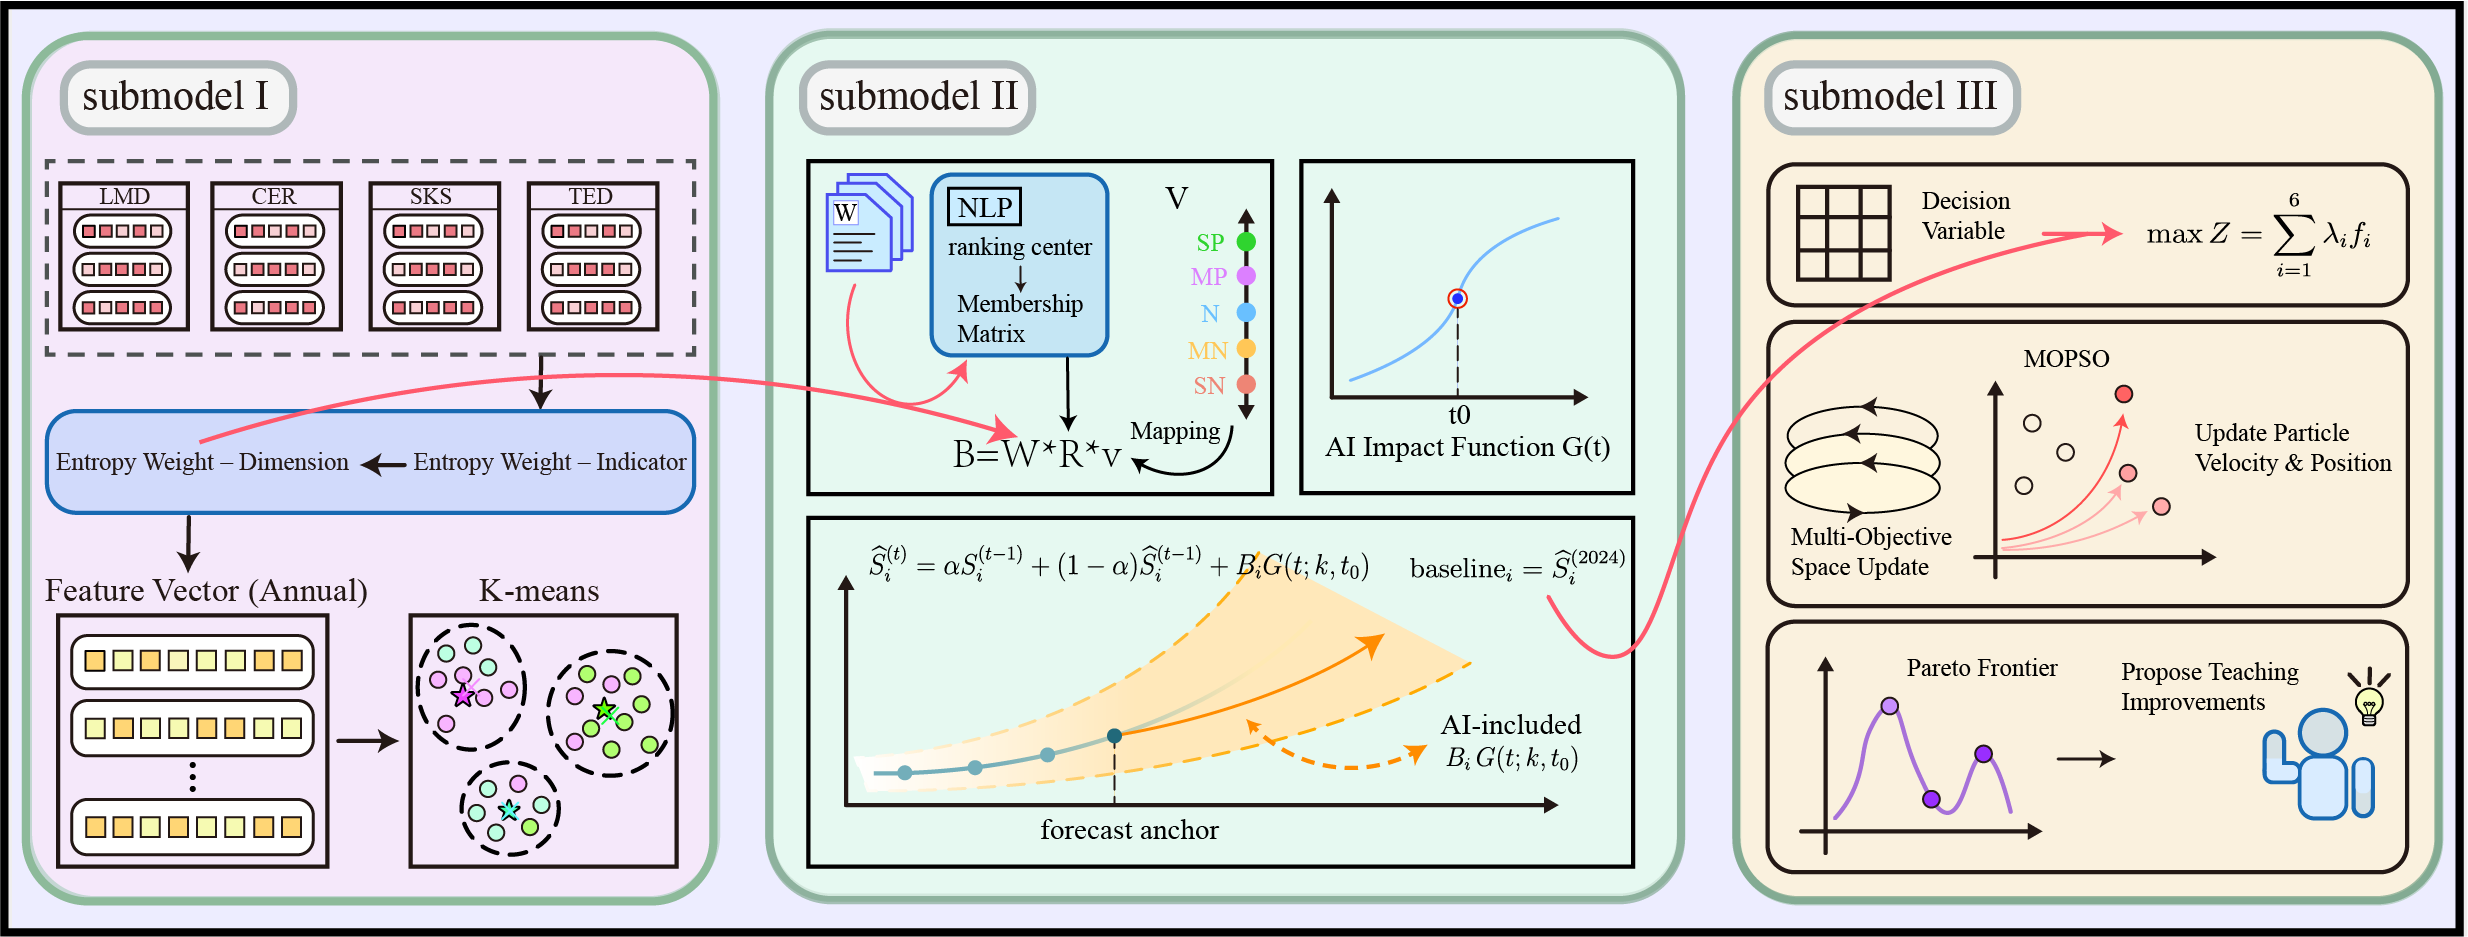
\includegraphics[width=\linewidth]{fig_framework.png}
\captionof{figure}{A two-dimensional t-SNE visualization of occupations colored by their occupational category labels (STEM, Trade, or Arts). The dashed circles in the figure represent clustering results.}
\label{fig_framework.png}
\end{center}






%%----------------------------------------------------------------------------------
%%----------------------------------------------------------------------------------
\section{Assumptions and Justifications}


\noindent\textbf{Assumption 1: Data Accuracy}\\
\noindent\textbf{Justification:} This paper relies on authoritative public data sources,including BLS\cite{BLS}, NCES\cite{NCES}, CSD\cite{CSD}, and O*NET\cite{ONET}.
These data serve as foundational inputs for both occupational and educational dimensions.
This paper assumes consistent statistical methodologies and continuity in indicator definitions and collection methods across long-term database updates. It further assumes no future major institutional adjustments or statistical method changes that would cause systematic reconfigurations of these methodologies.
Residual errors primarily manifest as random noise rather than systematic bias.
This framework does not alter the conclusions drawn from relative comparisons across occupations and years.

\medskip
\noindent\textbf{Assumption 2：The indicator system is comprehensive and disregards the impact of indicators without metrics.}\\
\noindent\textbf{Justification：}This study employs a multidimensional indicator system.
The system covers core dimensions including labor demand, economic returns, skill structure, and technology dependency.
The indicator system is used to characterize occupational differences and evolutionary patterns.
This study assumes that excluded variables have a limited impact.
These variables contribute marginally to the final comprehensive evaluation and optimization conclusions.
They will not cause a systemic reversal in decision-making direction.



\medskip
\noindent\textbf{Assumption 3：The impact of generative AI will gradually intensify as it becomes more widespread, eventually stabilizing.}\\
\noindent\textbf{Justification：}The development of new technologies typically unfolds in three distinct phases:
adoption, diffusion, and maturity.
This paper applies this framework to project the trajectory of generative AI's impact.
Its influence on occupational tasks and skill requirements intensifies as adoption rates rise.
Upon reaching maturity, the impact's intensity gradually stabilizes.
This model enables future scenario analysis to capture temporal dynamics,
avoiding the simplistic view of impact as a one-time, sudden transformation.

\medskip
\noindent\textbf{Assumption 4：Institutional reforms can be approximated by a small number of continuous proportional variables.}\\
\noindent\textbf{Justification：}To ensure the model's operational feasibility, this paper describes training programs that use continuous variables, such as proportions of course modules and enrollment changes. It assumes that, within budgetary and structural constraints, the direction of these variables' effects on objectives—including employability, learning quality, inclusivity, resource utilization, and ethical compliance—remains stable. Simultaneously, the underlying mechanisms are interpretable. Consequently, the multi-objective trade-off results can serve as a reference for policy and management-level resource allocation decisions.


%%----------------------------------------------------------------------------------
%%----------------------------------------------------------------------------------
\section{Data Sources and Preprocessing}

\subsection{Data Sources}
\noindent To ensure traceability and reproducibility of conclusions, as shown in Table \ref{tab:data_sources_cn}, this paper uniformly uses four authoritative public databases as its foundational data sources. These databases comprehensively cover labor market outcomes, higher education supply and student outputs, and occupational-level task and skill profiles, thereby supporting subsequent clustering, comprehensive evaluation, and scenario analysis. To ensure traceability and reproducibility of conclusions, as shown in Table \ref{tab:data_sources_cn}, this paper uniformly uses four authoritative public databases as its foundational data sources. These databases comprehensively cover labor market outcomes, higher education supply and student outputs, and occupational-level task and skill profiles, thereby supporting subsequent clustering, comprehensive evaluation, and scenario analysis.

\noindent\textbf{Labor Market and Compensation(BLS)}
The U.S. Bureau of Labor Statistics (BLS) provides occupational-level employment and wage statistics (such as the OEWS system), which can be used to measure employment levels, compensation, and trends over time for occupations. It serves as the core source for the labor-demand and income-return indicators in this paper.

\noindent\textbf{Institutional and Enrollment Statistics(NCES} The National Center for Education Statistics (NCES) provides institutional-level information and annual statistics for colleges, universities, and vocational institutions through systems such as IPEDS. This data characterizes institutional attributes and serves as a standardized key and background information source for linking education-end data.

\noindent\textbf{Educational Outcomes and Returns(CSD)} The U.S. Department of Education's College Scorecard database provides metrics at the institutional level and for select programs, including completion rates, debt and repayment, and post-graduation earnings. These metrics measure the economic returns and financial burdens of different educational pathways and support the assessment of "education-to-career" trajectories.

\noindent\textbf{Occupational Tasks and Skills(O*NET)} O*NET OnLine provides structured information at the occupational level, including task descriptions, skill and competency requirements, and technical skills. This paper utilizes this repository to construct occupational task and skill features, offering actionable proxy variables for characterizing occupations' potential exposure to generative artificial intelligence.

\begin{table}[ht!]
\centering
\caption{Overview of Data Sources and Their Roles in the Modeling Process}
\label{tab:data_sources_cn}
\renewcommand{\arraystretch}{1.15}
\setlength{\tabcolsep}{6pt}
\begin{tabularx}{\linewidth}{@{}l X X@{}}
\toprule
\textbf{Data Source} & \textbf{Content Provided} & \textbf{Purpose in This Paper} \\
\midrule
BLS\cite{BLS} & Occupational employment and wage statistics & Constructing labor demand and compensation return metrics \\
NCES\cite{NCES} & Institutional attributes, enrollment, and outcome statistics & Characterizing institutional features and standardizing educational data connections \\
CSD\cite{CSD} & Completion rates, debt, graduate earnings, etc. & Evaluating educational pathway returns and affordability \\
O*NET OnLine\cite{ONET} & Occupational tasks, competencies, and technical skills & Occupational task-skill mapping and Gen-AI exposure proxy metrics \\
\bottomrule
\end{tabularx}
\end{table}

\subsection{Preprocessing}
To ensure comparability across different data sources and years, this study employs a two-step cleaning and missing value handling process for the original occupational data sample. First, occupations with fewer than 50 employed individuals are excluded to avoid instability in the assessment caused by small sample sizes. Second, a stratified approach to missing data was applied: a threshold for the missing rate was first set at the occupational level to screen samples. If the missing rate for a key indicator in a given occupation exceeded 10\%, it was deemed insufficient to support a reliable evaluation and was excluded. For occupations where the missing rate did not exceed the threshold, missing values were imputed using the indicator's mean within the same category and year. This approach minimizes sample size reduction while controlling noise, providing a consistent and reproducible data foundation for subsequent clustering analysis and comprehensive evaluation.











%%----------------------------------------------------------------------------------
%%----------------------------------------------------------------------------------
\section{Notations}
\begin{table}[ht!]
\centering
\caption{Notations}
\label{tab:notations_ultra_core_all_short}
\renewcommand{\arraystretch}{1.06}
\setlength{\tabcolsep}{6pt}
\begin{tabular}{p{0.22\linewidth} p{0.66\linewidth} p{0.08\linewidth}}
\hline
\noalign{\vskip 2mm}
\textbf{Symbols} & \textbf{Description} & \textbf{Unit} \\
\noalign{\vskip 2mm}
\hline

$\mathrm{score}_i^{(t)}$ & The composite score for occupation $i$ in year $t$ & -- \\
$\bar{\mathbf{w}}$ & The average dimension weight vector for the six-dimensional indicator system & -- \\
$K$ & The number of clusters and the number of occupational types & count \\

$\mathbf{R}_j$ & Membership matrix for occupation or type $j$ & -- \\
$\mathbf{v}$ & Influence level score vector & -- \\
$B_j^{(t)}$ & AI impact coefficient for occupation or type $j$ in year $t$ & -- \\
$G(t;k,t_0)$ & Macro AI impact intensity function in Logistic form & -- \\
$k,t_0$ & Logistic parameters: acceleration rate and inflection point year & year \\

 $\mathbf{x}$ & Institutional-level decision vector Course structure and enrollment adjustments & -- \\
$f_1,\dots,f_6$ & Six objective functions & -- \\
$\lambda_i$ & Objective weight coefficients & -- \\
$Z$ & Comprehensive objective function & -- \\
$l_i,h_i$ & Decision variable upper/lower bounds & -- \\
$\alpha,p,\beta$ & Key parameters: Constraint coupling, nonlinear sensitivity, and reduction coefficients & -- \\
$C_i$ & Unit cost coefficient & -- \\
$P_1,P_2$ & Constraint penalty terms & -- \\

\hline
\noalign{\vskip 1.5mm}
\end{tabular}
\end{table}



%%----------------------------------------------------------------------------------
%%----------------------------------------------------------------------------------
\section{Multi-objective optimization model}
\subsection{Sub-model I：Identification of Representative Occupations Based on Entropy Weighting and K-Means}

\subsubsection{Indicator Selection}
Submodel I first constructs a unified metric system to characterize the evolutionary features of different occupations over the past $n$ years against the backdrop of continuous Gen-AI development. Let $i = 1, \dots, m$ denote the occupation index, and $t \in {t_1, \dots, t_n}$ denote the year index. For each occupation-year observation, as shown in Table \ref{tab:dim_notations_all}, the study aggregates raw metric values across four dimensions: labor market demand, economic returns, skill structure, and technology dependency.



\newcommand{\DimHeader}[1]{%
  \noalign{\vskip 2pt}
  \cdashline{1-3}
  \noalign{\vskip 6pt}
  \multicolumn{3}{c}{\textbf{\textit{#1}}} \\
  \noalign{\vskip 6pt}
  \cdashline{1-3}
  \noalign{\vskip 2pt}
}

\captionsetup[table]{skip=12pt}



\begin{table}[ht!]
\centering
\caption{Indicator System of Submodel I}
\label{tab:dim_notations_all}
\renewcommand{\arraystretch}{1.08} % 原 1.15：略微收紧行距
\setlength{\tabcolsep}{30pt}       % 列间距保持不变
\begin{tabularx}{\linewidth}{@{}l X c@{}}
\toprule
\noalign{\vskip 1.2mm} % 原 2mm
\textbf{Symbol} & \textbf{Indicator Definition} & \textbf{Unit} \\
\noalign{\vskip 1.2mm} % 原 2mm
\midrule
\noalign{\vskip 0.6mm} % 原 1mm

\DimHeader{Dim1: Labor Market Demand (LMD)}
$\mathrm{LMD1}_{i}^{(t)}$ & Employment population size & — \\
$\mathrm{LMD2}_{i}^{(t)}$ & Employment growth rate & \% \\
$\mathrm{LMD3}_{i}^{(t)}$ & Unemployment rate & \% \\
\noalign{\vskip 0.8mm} % 原 1.2mm

\DimHeader{Dim2: Compensation and Economic Return (CER)}
$\mathrm{CER1}_{i}^{(t)}$ & Median annual salary & USD/year \\
$\mathrm{CER2}_{i}^{(t)}$ & Salary growth rate & \% \\
$\mathrm{CER3}_{i}^{(t)}$ & Income dispersion ratio & \% \\
$\mathrm{CER4}_{i}^{(t)}$ & Education-return ratio & \% \\
$\mathrm{CER5}_{i}^{(t)}$ & Middle-to-high income premium & \% \\
\noalign{\vskip 0.8mm} % 原 1.2mm

\DimHeader{Dim3: Skill Structure (SKS)}
$\mathrm{SKS1}_{i}^{(t)}$ & Share of high-skill positions & \% \\
$\mathrm{SKS2}_{i}^{(t)}$ & Skill update frequency & 1/year \\
\noalign{\vskip 0.8mm} % 原 1.2mm

\DimHeader{Dim4: Technology Dependence (TED)}
$\mathrm{TED1}_{i}^{(t)}$ & Digital tool adoption rate & \% \\
$\mathrm{TED2}_{i}^{(t)}$ & Automation potential index & - \\
$\mathrm{TED3}_{i}^{(t)}$ & Technology investment intensity & USD/year \\
$\mathrm{TED4}_{i}^{(t)}$ & Workflow standardization level & index \\
\noalign{\vskip 1.0mm} % 原 1.5mm
\bottomrule
\end{tabularx}
\end{table}



Due to significant data gaps in 2025, we collected data from over 200 positions spanning 2015 to 2024 to assess industry development over the past decade and assigned category labels to each occupation. To standardize units, we transformed the negative indicators $\mathrm{LMD3}_{i}^{(t)}$ and $\mathrm{CER3}_{i}^{(t)}$, then normalized the data using the min-max method. Building on this, the normalized data served two core objectives: first, integrating multidimensional metrics into a single annual composite score to ensure comparability across occupations and time periods and second, selecting representative occupations from each category by combining their current development levels with clustering characteristics.

To mitigate biases arising from subjective weighting, this paper employs the Entropy Weighting Method (EWM) to determine indicator weights and calculate the composite scores for each occupation. EWM assigns higher weights to indicators exhibiting greater dispersion within the "occupation-year" panel data, thereby providing stronger discriminative information to distinguish occupational differences. Assuming the entropy weight for the $j$th indicator, denoted as $w_j$, is calculated from the panel data, the annual composite score for occupation $i$ in year $t$ can be defined as

\begin{equation}
\mathrm{score}_i^{(t)}=\sum_{j=1}^{d} w_j\, x_{ij}^{(t)} .
\label{eq:score}
\end{equation}

By connecting the composite scores for each year of a given profession in sequence, one can obtain the multi-year composite score trajectory vector for that profession.

\begin{equation} 
\mathrm{score}_i = \big[\mathrm{score}_i^{(t_1)},\mathrm{score}_i^{(t_2)}, \dots, \mathrm{score}_i^{(t_n)}\big]. 
\end{equation}

\begin{center}

\includegraphics[width=0.7\linewidth]{MCM:ICM/Elbow_Method.png}
\captionof{figure}{Elbow Method for Determining the Number of Clusters}
\label{fig:Elbow_Method}
\end{center}

To identify representative occupational types, we performed cluster analysis based on the similarity of recent occupational score trajectories. Specifically, we used ${score}_i$ as the feature vector for each occupation $i$ and applied K-means clustering to the feature vector set $\{score_i\}$ for all occupations. This divided occupations into K groups, revealing distinct distributions for STEM, trade, and arts occupations. Finally, we selected the most representative occupations from each cluster by considering both the proportion of occupations within each cluster and the distance of each occupation from the cluster center. As shown in \ref{fig: Elbow_Method}, the elbow method determined the optimal number of clusters to be 3.



\begin{center}

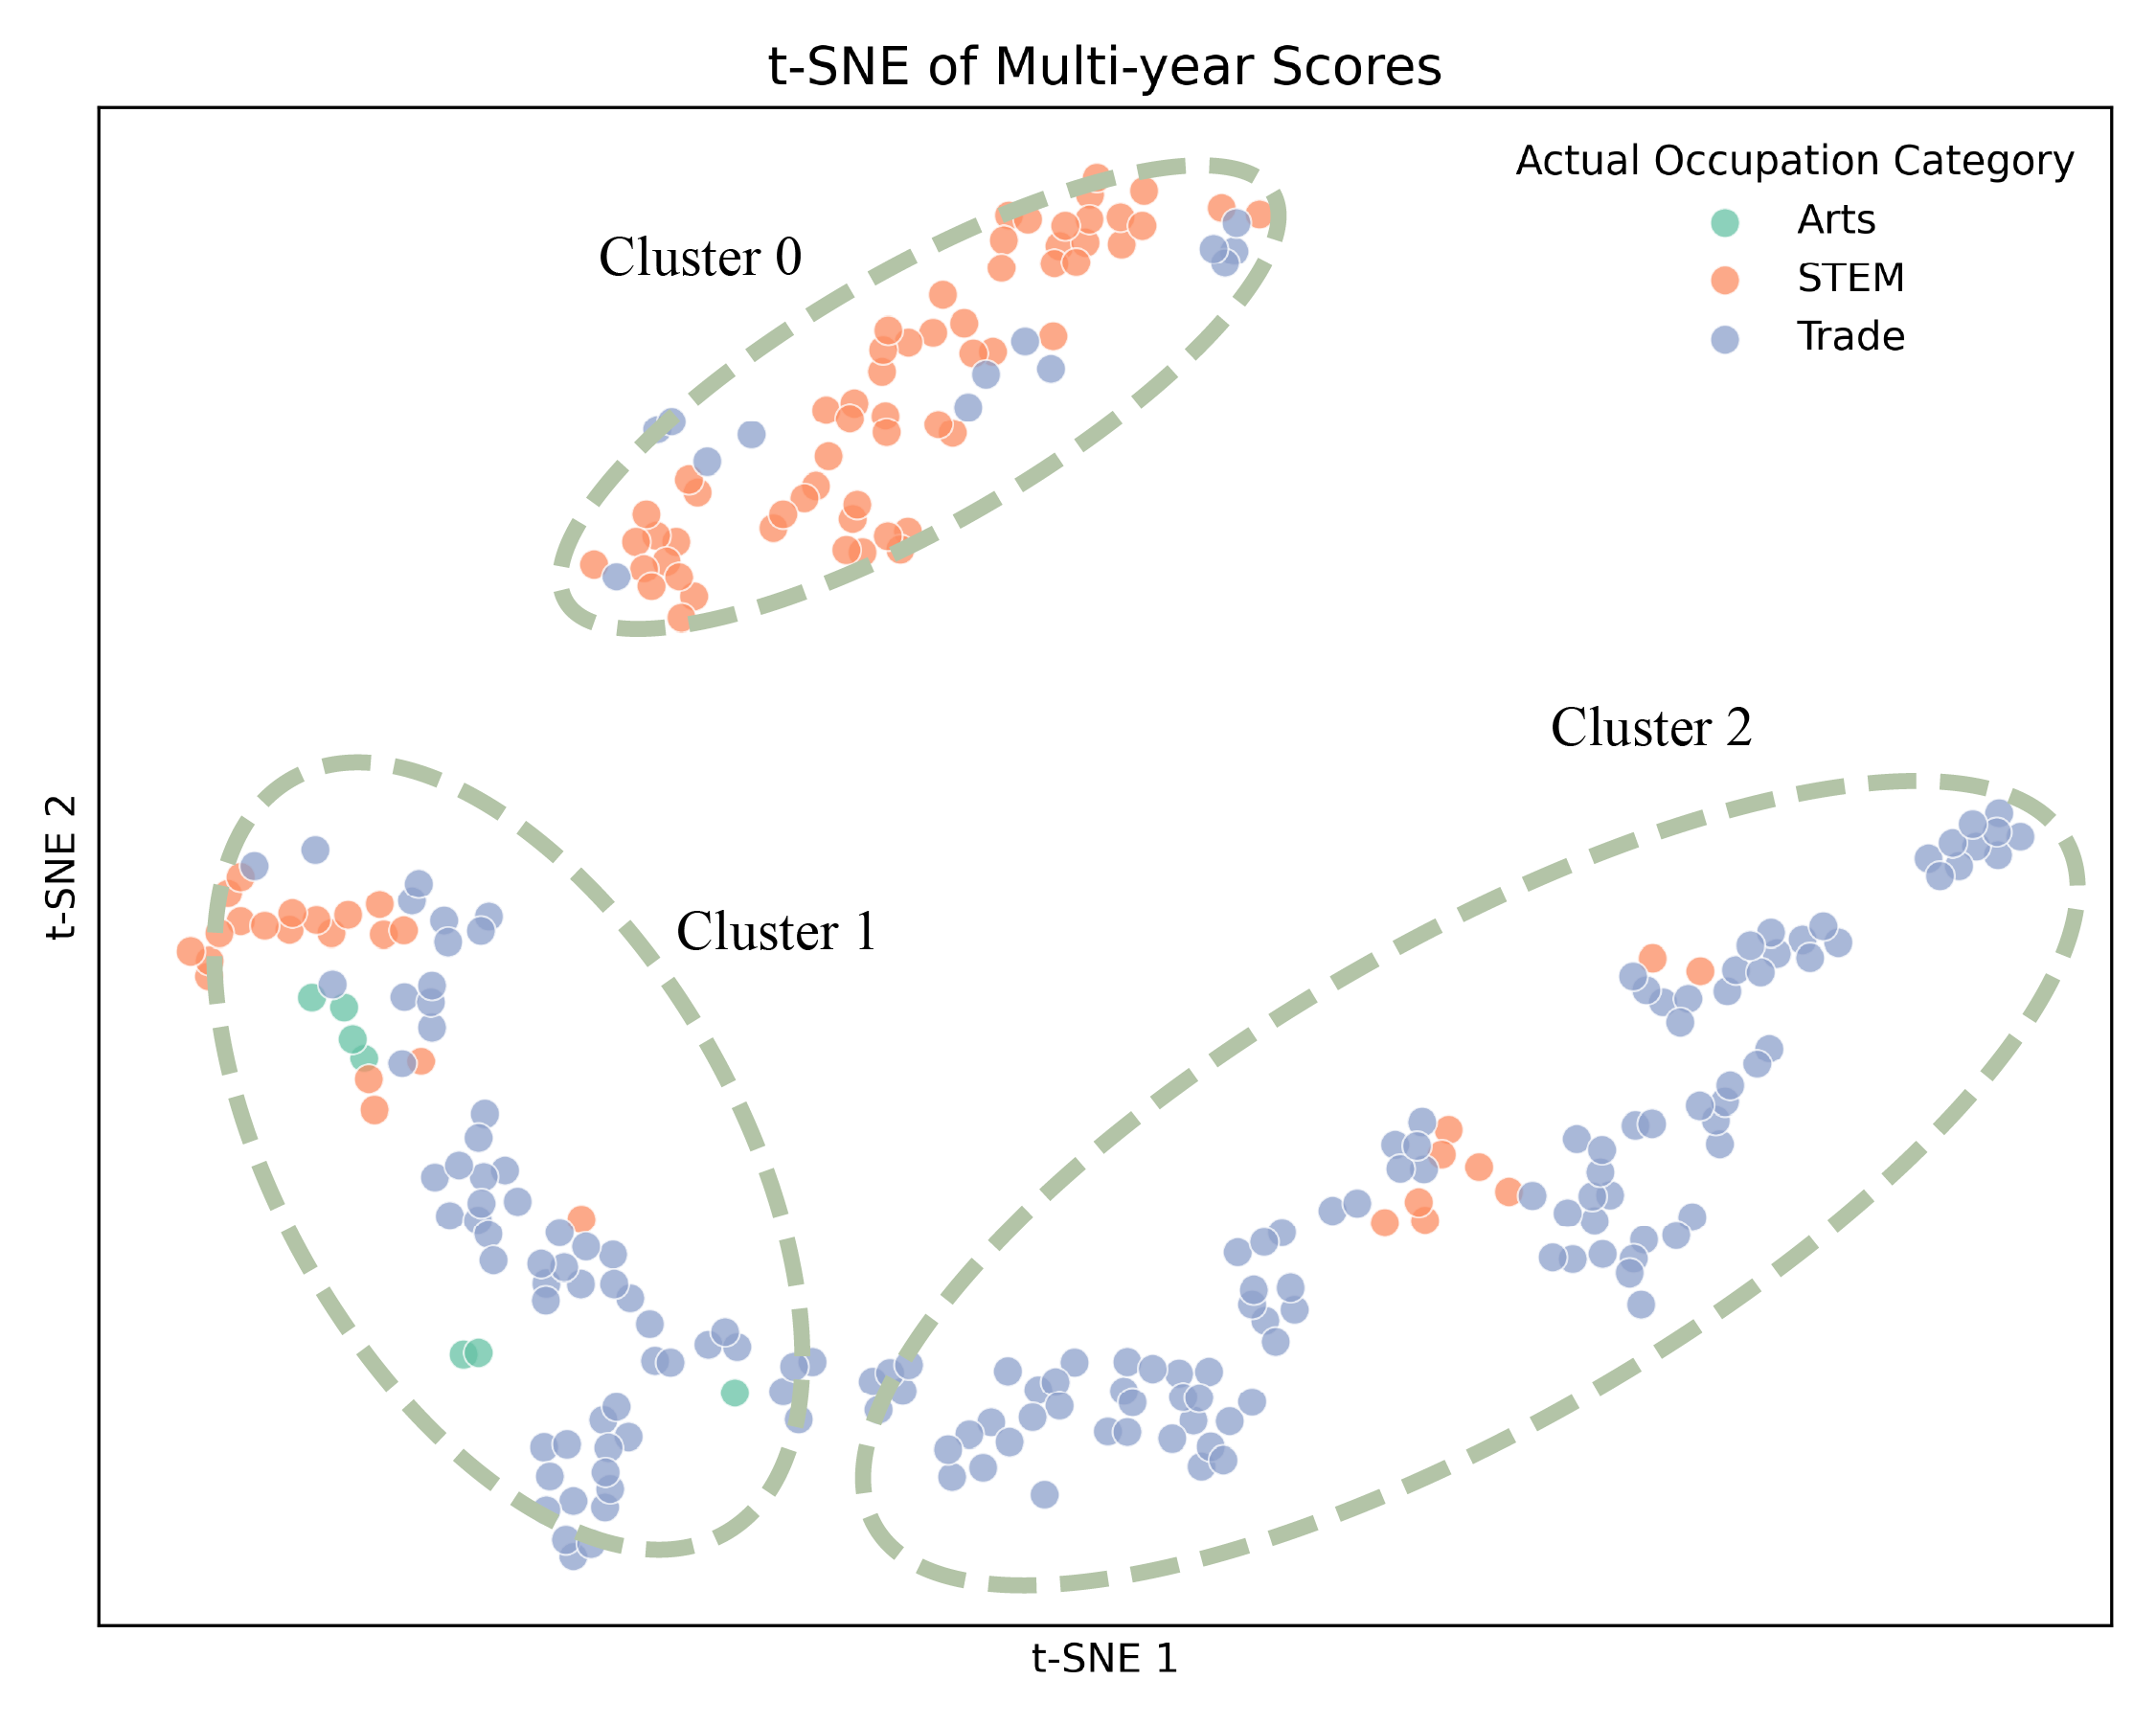
\includegraphics[width=0.7\linewidth]{fig_tsne_Kmeans.png}

\captionof{figure}{A two-dimensional t-SNE visualization of occupations colored by their occupational category labels (STEM, Trade, or Arts). The dashed circles in the figure represent clustering results.}

\label{fig:tsne_clusters}

\end{center}


\subsubsection{Results: Type Explanation, Representative Occupations, and Trend Forecasts}
\noindent To visually represent the clustering structure in the high-dimensional composite indicator space, this paper employs the t-SNE algorithm to map occupational samples onto a two-dimensional plane for visualization, as shown in Figure \ref{fig:tsne_clusters}. The three distinct clusters of data points exhibit clear separation boundaries, indicating that within the feature space defined by composite indicators, different occupational types form relatively stable clustering structures rather than continuous distributions along a single dimension. Based on the clustering results, this paper selects the job within each cluster that is closest to the cluster center and belongs to an occupational category with a large proportion within the cluster group as the representative for each category. Ultimately, the first cluster is represented by Railway Maintenance Worker (trade category), the second cluster by Management Analyst (STEM category), and the third cluster by Graphic Designer (arts category).

\begin{center}

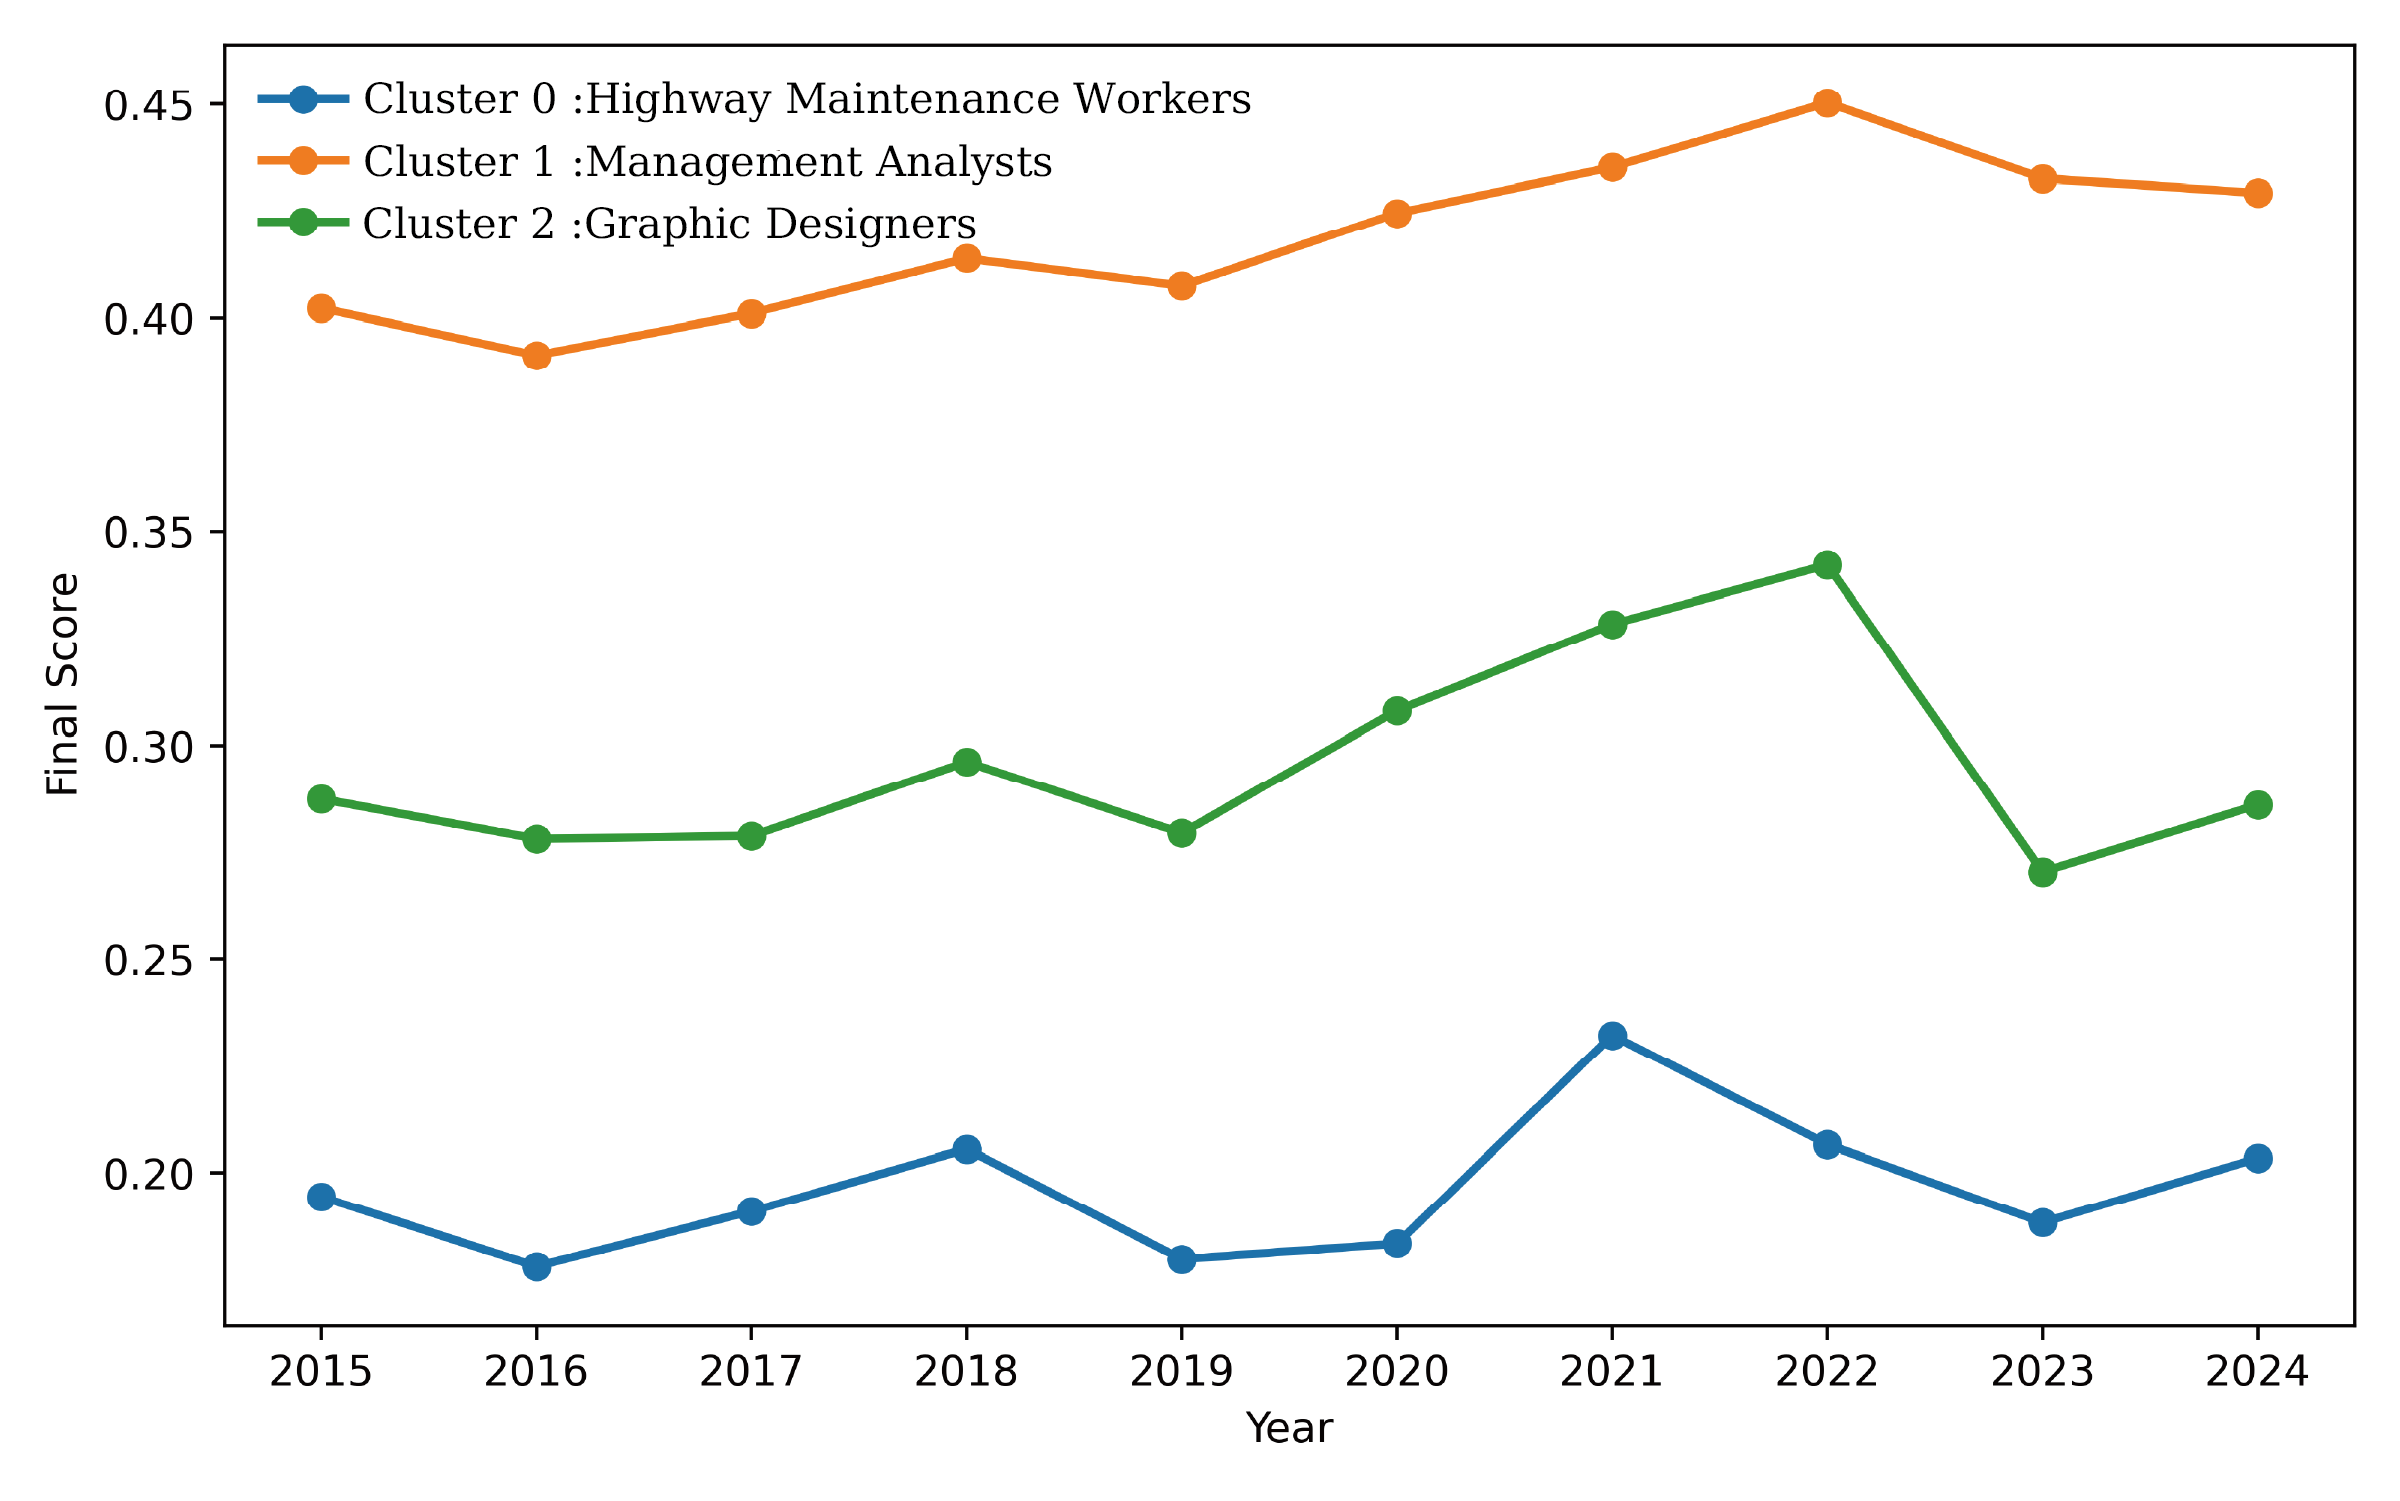
\includegraphics[width=0.7\linewidth]{fig_year_scores.png}

\captionof{figure}{Annual Composite Score Trend Chart for Three Representative Occupations.}

\label{fig:tsne_clusters}

\end{center}

As shown in the figure, the composite scores for the three occupations we selected exhibit stable and clearly tiered long-term trends, accompanied by normal annual fluctuations. Management analysts have maintained higher composite scores for many years, demonstrating stronger demand signals and superior educational returns. Railway maintenance workers show relatively low composite scores, with high exposure to automation and slow skill updates. Graphic designers rank in the middle but face the most significant future impact from AI, with the greatest demand divergence between high-end and low-end roles.

\begin{table}[H]  % 将 [htbp] 改为 [H]，强制固定位置
\centering
\caption{Occupational Type: Explanatory Summary, and Representative Occupations.}
\label{tab:cluster_profile}
\begin{tabular}{p{0.12\linewidth} p{0.52\linewidth} p{0.12\linewidth} p{0.18\linewidth}}
\hline
Cluster & Interpretation & Code(Source: BLS\cite{BLS}) & Representative occupation \\
\hline
C0 (Trade) &
Large workforce but slow growth; moderate educational returns; low-to-medium skill dependency with slow skill renewal. Routine, experience-driven jobs face higher substitution risks in generative AI contexts. &
47--4051 &
Railway Maintenance Worker \\
\hline
C1 (STEM) &
Rapid job growth, high compensation, strong educational returns, frequent digital tool usage, high technology investment intensity, and a high proportion of high-skill positions. Strong human capital and "technology complementarity" maintain a high composite score and a low risk of job displacement. &
13--1111 &
Management Analyst \\
\hline
C2 (Arts) &
Significant income volatility and pay disparities; divergent educational returns; uneven technology reliance with low automation risk; overall moderate score, but higher uncertainty and more pronounced tail risks. &
27--1024 &
Graphic Designer \\
\hline
\end{tabular}
\end{table}

Ultimately, we analyzed the characteristics of different job categories using Submodel I, selecting railway maintenance workers, management analysts, and graphic designers as representatives of the trade, STEM, and arts occupational categories, respectively. Subsequent models examined the future impact of Gen-AI on these professions and the direction for higher education institutions to adjust their training programs.

%%----------------------------------------------------------------------------------
\subsection{Sub-model II:}
\subsubsection{Fuzzy Comprehensive Evaluation of Gen-AI Impact}

The impact of Gen-AI varies significantly across different occupations. Some professions will experience rapid growth alongside AI development, while others will face relatively limited influence. Still others may face partial replacement by artificial intelligence. These shifts in career development patterns will directly influence talent cultivation programs within relevant disciplines at higher education institutions. To clarify future trends across occupations and provide a basis for higher education institutions to formulate talent development reform strategies for AI-impacted industries, this paper employs the Fuzzy Comprehensive Evaluation (FCE) method. Based on multidimensional foundational data from Submodel I, we conduct a quantitative assessment of AI's impact across occupations along multiple dimensions. We derive the evaluation set from Submodel I.
\begin{equation} 
U=\{\mathrm{Dim1},\mathrm{Dim2},\mathrm{Dim3},\mathrm{Dim4}\}.
\end{equation}

Similarly, we adopt the annual weights from Submodel I to obtain the historical weight set.
\begin{equation} 
W^{(t)}=\big[w_1^{(t)}, w_2^{(t)}, w_3^{(t)}, w_4^{(t)}] .
\end{equation}

We have established five possible evaluation outcomes.
\begin{equation} 
\begin{aligned}
V=\{\,&\text{Strong Positive Impact, Moderate Positive Impact, Neutral Impact,} \\
&\text{Moderate Negative Impact, Strong Negative Impact}\},
\end{aligned}
\end{equation}
Assign them scores from the set $\{0.2, 0.1, 0, -0.1, -0.2\}$, enabling us to quantify the overall impact. Simultaneously, define the midpoints of each grade as $\{0.08, 0.04, 0, -0.04, -0.08 \}$.

为减少隶属度矩阵$R$完全依赖人工设定的主观性，我们利用关于未来工作变化的研究\cite{FreyOsborne2017,McKinseyGenAIPotential,NBERWorkplaceGenAI,OECDEmploymentOutlook2023,OECDThreeDrivers}[！插入文献！Ai L B Y, Ai W B. GPTs are GPTs: An Early Look at the Labor Market Impact Potential of Large Language Models By admin No Comments[J]. 2023. and so on（笔记p9）]，使用Natural Language Processing (NLP)技术提取文献关键词，并与我们为每个维度设定的关键词对照，衡量职业$i$的$j$维度受到的影响
\begin{equation} 
y_{ij}=\frac{\mathrm{positive\_word}-\mathrm{negative\_word}}{\mathrm{total\_word}}.
\end{equation}
The numerator of this ratio represents the difference between positive and negative keywords, serving to measure whether Gen-AI exerts a positive or negative influence on the future. The denominator accounts for variations in corpus length. Ultimately, we employ the $y_{ij}$ mapping to reflect the membership matrix of AI's impact across various dimensions.

Based on an analysis of existing research and evaluation results, we use the triangular membership function.
\begin{equation}
r_{jd}^{(i)}=\max\!\left(1-\frac{|y_{ij}-c_d|}{d_0},\,0\right)
\end{equation}
to map text data onto the membership matrix $\mathbf{R}_{i}\in[0,1]^{4\times 5}$. Here, $r_{jd}^{(i)}$ represents the probability that the AI's influence on dimension $j$ of occupation $i$ ultimately falls within level $d$. $c_d$ denotes the level's center, and $d_0$ is the half-width, set to 0.4 in this scenario.

As $y_{ij}$ approaches the class center $C_d$, its membership to class $d$ increases and linearly decays with distance. When deviation exceeds half-width $d_0$, membership is truncated to 0, thereby suppressing non-physical contributions from distant classes. Building upon this, we perform minor manual calibration on $\mathbf{r}_{jd}^{(i)}$ by integrating category scores from Submodel I with occupational reality constraints. This corrects potential biases in textual evidence while ensuring consistency and interpretability between impact directions and occupational profiles.


Based on the NLP results, membership functions, and manually fine-tuned outputs, we present membership matrices for the Trade, STEM, and Arts occupational categories. These matrices will be used to quantify the comprehensive impact in subsequent analyses:

\begin{align}
\mathbf{R}_{\text{trade}} &=
\begin{bmatrix}
0.05 & 0.15 & 0.60 & 0.15 & 0.05\\
0.05 & 0.10 & 0.65 & 0.15 & 0.05\\
0.10 & 0.15 & 0.60 & 0.10 & 0.05\\
0.05 & 0.10 & 0.70 & 0.10 & 0.05
\end{bmatrix}, \label{eq:R_trade}\\
\mathbf{R}_{\text{STEM}} &=
\begin{bmatrix}
0.35 & 0.40 & 0.15 & 0.07 & 0.03\\
0.30 & 0.45 & 0.15 & 0.07 & 0.03\\
0.40 & 0.40 & 0.12 & 0.06 & 0.02\\
0.55 & 0.30 & 0.10 & 0.04 & 0.01
\end{bmatrix}, \label{eq:R_stem}\\
\mathbf{R}_{\text{arts}} &=
\begin{bmatrix}
0.08 & 0.22 & 0.20 & 0.30 & 0.20\\
0.06 & 0.20 & 0.25 & 0.29 & 0.20\\
0.20 & 0.25 & 0.30 & 0.20 & 0.05\\
0.30 & 0.40 & 0.22 & 0.06 & 0.02
\end{bmatrix}. \label{eq:R_arts}
\end{align}

\subsubsection{AI Impact Function Fitting and Parameter Calibration}

The impact of AI on occupations is also linked to the pace of AI technological advancement and its level of adoption. Considering that the diffusion of generative AI typically follows a phased pattern—slow start, rapid acceleration, and eventual saturation—we employ a Logistic diffusion function to characterize the temporal evolution of macro-level AI impact intensity. This serves as the unified temporal driver for Submodel II:
\begin{equation}
G(t;k,t_0)=\frac{1}{1+\exp\!\left[-k\left(t-t_0\right)\right]}.
\label{eq:logistic_shock}
\end{equation}
Here, $t$ denotes the calendar year, $k$ represents the diffusion acceleration rate, and $t_0$ is the inflection point year satisfying $G(t_0;k,t_0)=0.5$, corresponding to the central moment of transition from low-intensity to high-intensity shocks. Based on relevant research\cite{METR2025ForecastAI}, we fitted the parameters of the AI shock function to $k=0.8$ and $t_0=2027$.

\subsubsection{Time Series Models Predict Future Career Development}

In Submodel I, we observe that while different occupations exhibit distinct current development trajectories, they maintain relative stability. Here, we conduct an in-depth analysis of developmental patterns across occupations and combine this with AI's influence to jointly forecast their future trajectories. Given that we have data only from the past decade, Submodel II employs smoothing time-series analysis to estimate the baseline trend of $score_i$ over the last 10 years. Since the impact of the AI shock function remains below 0.1 until 2024, we can conclude that the baseline data has not been affected by AI. The time series forecasting steps are as follows:

\noindent \textbf{(1) Single Exponential Smoothing of Baseline Sequences and Parameter Selection.}
Based on Submodel I, let $S_i^{(t)}$ denote the composite score for occupation $i$ in year $t$. The recursive form of exponential smoothing is given by
\begin{equation}
\widehat{S}_i^{(t)}
=\alpha S_i^{(t-1)}+(1-\alpha)\widehat{S}_i^{(t-1)},
\qquad 0<\alpha<1.
\label{eq:ses_S_cn}
\end{equation}
Where $\widehat{S}_i^{(t)}$ represents the single exponential smoothing estimate for occupation $i$ in period $t$, $S_i^{(t)}$ denotes the actual observed value for occupation $i$ in period $t$, and $\widehat{S}_i^{(t-1)}$ is the single exponential smoothing estimate for occupation $i$ in period $t-1$; $\alpha$ is the exponential smoothing coefficient, with values ranging from $0<\alpha<1$. It controls the weight allocation between the current actual observation and the previous smoothed estimate in the current smoothing result. The magnitude of the smoothing coefficient $\alpha$ directly determines the weight allocation: A larger $\alpha$ increases the weight of the current actual observation, making the smoothed result more responsive to recent data changes; A smaller $\alpha$ increases the weight of the previous period's smoothed estimate, enhancing the overall stability of the smoothed result.
To avoid the subjective setting of the smoothing coefficient, this paper defines a candidate set $\alpha \in \{0.1, 0.2, 0.3, 0.4, 0.5\}$. Selection is performed using backtesting error: using $t \in [2015, 2019]$ as the training interval yields $\widehat{S}_i^{(2019)}$, which serves as the baseline anchor for the validation interval.
\begin{equation}
\mathrm{baseline}_{i}=\widehat{S}_i^{(2019)},
\end{equation}
then calculates the mean absolute error over $t\in[2020,2024]$
\begin{equation}
\mathrm{MAE}(\alpha)=\frac{1}{5}\sum_{t=2020}^{2024}\left|S_i^{(t)}-\mathrm{baseline}_{i}\right|,
\label{eq:mae_alpha}
\end{equation}
Select $\alpha$ that minimizes $\mathrm{MAE}(\alpha)$ as the optimal smoothing coefficient.

After obtaining the optimal $\alpha$, this paper re-smooths the entire historical interval $t\in[2015,2024]$ to form a prediction baseline, and uses
\begin{equation}
\mathrm{baseline}_{i}=\widehat{S}_i^{(2024)}
\end{equation}
as the baseline for future predictions without AI impact.

\noindent \textbf{(2) Weight stabilization and the prolongation of occupational shock magnitude.}
To mitigate the impact of interannual fluctuations in weights on long-term forecasts, this paper employs the average weights from the past decade:
\begin{equation}
\bar{\mathbf{w_i}}=\frac{1}{10}\sum_{t=2015}^{2024}\mathbf{w_i}^{(t)}.
\label{eq:wbar}
\end{equation}
yielding the average weight set $\overline{W}=[w_1,w_2,w_3,w_4]$.
Accordingly, the AI impact magnitude for occupation $i$ is defined as the long-term structural coefficient:
\begin{equation}
B_i={\overline{W}}\mathbf{R}_i\mathbf{V},
\label{eq:B_longrun}
\end{equation}
where $B_i$ denotes AI's ultimate overall impact on the future of occupation $i$. This definition insulates the impact magnitude from short-term annual fluctuations, with temporal variation primarily driven by the macro-diffusion term $G(t;k,t_0)$.

\noindent \textbf{(3) AI-adjusted forecast.}
Combining the Logistic macro-shock intensity function $G(t;k,t_0)$ from the previous subsection, the AI-adjusted forecast value for occupation $i$ in future year $t$ is defined as
\begin{equation}
S_{i,\mathrm{future}}^{(\tau)}
=\underbrace{\mathrm{baseline}_{i}}_{\text{No AI baseline}}
+\underbrace{B_i\,G(t;k,t_0)}_{\text{AI Adjustment Items}},
\label{eq:ai_adjusted_forecast_cn}
\end{equation}
When AI is in its early diffusion phase, $G(t;k,t_0)$ is small, and the predicted values approach the baseline without AI. As AI approaches the mature diffusion phase, $G(t;k,t_0)\to 1$, and the prediction offset is primarily determined by the sign and magnitude of $B_i$. Consequently, the model can characterize both net enhancement and net substitution pathways across different occupations within a single framework, producing standardized results suitable for scenario and sensitivity analyses.

\noindent \textbf{(4) Initialization settings.}
To ensure computational feasibility of the recursive process, the smoothing sequence is initialized with
${S}_j^{(2015)}=S_j^{(2015)}.$ This initialization remains robust under limited annual samples and avoids introducing additional uninterpretable free parameters.



%%----------------------------------------------------------------------------------
\subsection{Sub-model III：}

At the institutional level, to address the reshaping of job tasks and skill requirements by generative AI, this paper selects one representative program from each of three educational pathways as its research subjects. These correspond to the training directions for technical-skilled, data-analytical, and creative-design talent, specifically including: - Railway Engineering Technology at Vocational College A, - Business Analytics at Comprehensive University B, - and Visual Communication Design at Art College C.


Centering on three cultivation programs, we have developed a multi-objective decision-making framework for program selection and resource allocation that encompasses six optimization goals. The first is the core objective: maximizing graduate employability within given constraints, reflecting the program's comprehensive contribution to labor-market alignment and career sustainability. The second objective optimizes program enrollment scale to achieve supply-demand alignment while managing capacity risks. The third balances the learning efficiency and outcomes of GENAI, emphasizing enhanced learning output quality within limited time and cost investments. The fourth enhances knowledge accessibility and institutional resource utilization, balancing educational equity with resource allocation efficiency. Fifth, controlling ethical risks and ensuring content originality by incorporating academic integrity, data compliance, and generative content traceability into constraint and penalty mechanisms. Sixth, reducing societal resource waste by mitigating externalities like energy consumption associated with GenAI usage at a higher level. These objectives collectively serve as the evaluation benchmarks for subsequent multi-objective optimization modeling and policy-scenario comparisons.

\subsubsection{Multi-objective optimization}
\noindent\textbf{Objective 1: Maximize graduate employability.}
To measure the overall alignment of the program with the labor market, we construct employability indicators based on quantifiable training elements selected across four dimensions of Submodel I: labor market demand, economic returns, skill structure, and technology dependency. These indicators are: proportion of industry-academia collaboration courses $x_1$, proportion of core curriculum courses $x_2$, proportion of skills certification training courses $x_3$, and proportion of practical training courses $x_4$, weighted by Dim1 to Dim4. The expression for Objective 1 is as follows:
\begin{equation}
f_1=\sum_{i=1}^{4} w_i x_i 
\end{equation}

\noindent\textbf{Objective 2: Optimize program enrollment scale.}
To align enrollment size with labor demand, this paper uses the employment-growth-rate indicator $\mathrm{LMD2}$ from Submodel I as the market-demand signal. Simultaneously, indicator $x_5$ is set as the rate of change for the program's enrollment size. Intuitively, the closer $x_5$ is to $\mathrm{LMD2}$, the lower the risk of supply-demand mismatch. Therefore, we establish the expression for Objective 2:
\begin{equation}
f_2=-\bigl|x_5-\mathrm{LMD2}\bigr|
\end{equation}

\noindent\textbf{Objective Three: Balancing Learning Efficiency and Learning Outcomes.}
To simulate the double-edged impact of digital tools on the learning process, this paper uses the digital tool usage rate indicator $\mathrm{TED1}$ from Model I as a benchmark for reasonable levels of tool dependency. Let $x_6$ denote the project's Gen-AI usage intensity, which can be measured by AIGC intervention rate or AI usage frequency in assignments. Excessively high $x_6$ may lead to superficial learning and inflated competency, while excessively low $x_6$ may reduce learning efficiency and tool literacy. Therefore, this paper characterizes the principle of moderate usage through deviation penalties.
\begin{equation}
f_3=-\bigl(x_6-\mathrm{TED1}\bigr)^2
\end{equation}

\noindent\textbf{Objective 4: Enhance Knowledge Accessibility and Institutional Resource Utilization.}
Programs forced to reduce enrollment due to Gen-AI disruption can compensate for underutilized resources by expanding public liberal arts courses. These courses serve the broader public, disseminating knowledge while generating revenue through moderate fees. This paper uses the proportion of public liberal arts courses, denoted as $x_7$, as an indicator and characterizes this objective in terms of positive utility:
\begin{equation}
f_4= x_7\bigl[\max(-x_5,0)\bigr]^p
\end{equation}
For institutions with significant enrollment reductions, the model increases the value of $x_7$ to minimize waste of teaching resources. For programs in expansion phases, we require them to focus on enhancing their teaching and employment capabilities. Therefore, assuming sufficient budget, the target for programs in expansion phases is set to 0. The power index $p$ determines the impact of the magnitude of enrollment reduction on the target for offering general education courses.

\noindent\textbf{Objective 5: Control ethical risks and ensure content originality.}
Intuitively, increased AI usage heightens risks of plagiarism, unclear attribution, and ethical violations. Let $x_8$ denote the proportion of training courses dedicated to AI ethics and original content standards. We aim to mitigate these risks through standardized training while enhancing awareness of originality. To simultaneously reflect the positive effects of training investment and the adverse effects of high-intensity AI usage, this paper defines Objective 5 as
\begin{equation}
f_5=x_8(1-x_6)
\end{equation}

\noindent\textbf{Objective 6: Reduce waste of social resources.}
The use of AI increases energy and water consumption. We characterize the resource-saving effect using the linear term $x_6$ and introduce the discount factor $\beta$ to represent the relative weight of this effect. The expression for Objective 6 is:
\begin{equation}
f_6=-\beta x_6
\end{equation}
Although we encourage students to consider environmental factors when using AI, this should not be the primary constraint on AI adoption. Therefore, $\beta$ is set to 0.3. This conservative value reflects AI's efficiency gains while avoiding excessive suppression of educational innovation.


\noindent\textbf{Comprehensive Objective Function}
To uniformly balance the six objectives, this paper employs the weighted sum method to construct the overall utility function:
\begin{equation}
\max Z=\sum_{i=1}^{6}\lambda_i f_i
\end{equation}
where the weight $\lambda_1$ for the primary objective $f_1$ is set to 0.5, and the weights for the remaining objectives are set to 0.1.
The constraints are defined as:
\begin{equation}
\text{s.t.}
\begin{cases}
l_i\le x_i\le h_i,\qquad i=1,2,\dots,8 \\
x_1+x_2+x_3+x_4+x_7+x_8\le 1\\
C_1x_1+C_2x_2+C_3x_3+C_4x_4+C_7x_7+C_8x_8\le C_0
\end{cases}
\end{equation}
Among them, the first equation represents the boundary constraints for each variable; the second equation ensures the feasibility of the curriculum structure through proportional constraints; the third equation imposes a feasible budget-domain constraint, limiting the budget for each course type not to exceed the total budget. Regarding boundary constraints, for variables $x_1$ through $x_6$, we set constant upper and lower bounds based on typical scenarios. Since program expansion may divert resources from general education courses, we set the upper limit for $x_7$ based on the scale of the course expansion. For $x_8$, as AI risks are tied to AI usage intensity, educational institutions should ensure a minimum investment in AI ethics courses, thus linking its lower limit to AI usage intensity. Based on the above descriptions, we design the upper and lower limits for variables across three projects in three educational institutions:

\medskip
\noindent\textbf{(1) Trade school $A$ Railroad Engineering Technology：}
\[
\mathbf{l}^{(A)}=
(0.05,\ 0.2,\ 0.05,\ 0.05,\ -0.25,\ 0,\ 0,\ \alpha x_6)
\]
\[
\mathbf{h}^{(A)}=
(0.5,\ 1,\ 0.5,\ 0.5,\ 0.25,\ 1,\ 0.5-x_7[\max(0,x_5)]^{p},\ 0.3)
\]

\medskip
\noindent\textbf{(2) University $B$ Business Analytics：}
\[
\mathbf{l}^{(B)}=
(0,\ 0.5,\ 0,\ 0,\ -0.25,\ 0,\ 0,\ \alpha x_6)
\]
\[
\mathbf{h}^{(B)}=
(0.3,\ 1,\ 0.3,\ 0.3,\ 0.25,\ 1,\ 0.5-x_7[\max(0,x_5)]^{p},\ 0.15)
\]

\medskip
\noindent\textbf{(3) Arts school $C$ Graphic Design：}
\[
\mathbf{l}^{(C)}=
(0.05,\ 0.3,\ 0.05,\ 0.05,\ -0.25,\ 0,\ 0,\ \alpha x_6)
\]
\[
\mathbf{h}^{(C)}=
(0.3,\ 1,\ 0.5,\ 0.5,\ 0.25,\ 1,\ 1-x_7[\max(0,x_5)]^{p},\ 0.3)
\]
Among these, $\alpha$ is the coefficient regulating the impact of AI intensity on AI ethics courses, set at 0.3; $p$ is the coefficient measuring the impact of enrollment expansion on public liberal arts courses, set at 1.5.

For constraint 3, $C_i$ represents the cost associated with course $x_i$, and $C_0$ denotes the project's total annual budget. The project's total budget is determined by enrollment scale and current employment status. We stipulate that
\[
\mathbf{C}=
(15,\ 5,\ 10,\ 10,\ -2,\ 1)
\]
After normalizing the baseline in Model II, calculate the total budget adjusted for enrollment size and industry conditions.
\[
\mathbf{C_0}=
20(1+x_5)baseline
\]

\subsubsection{PSO for Solving the Curriculum Allocation Problem}
To solve the aforementioned optimization model in continuous space, this paper employs a particle swarm optimization algorithm to search for the optimal course allocation ratio. Each particle represents a feasible solution.
$\mathbf{X}=(x_1,\dots,x_8)$，
and use the composite objective value $Z$ as the fitness function:
\[
\mathrm{fitness}(\mathbf{X})=Z
\]

Where $\eta=10$. For the budget constraint, define the penalty term
\[
P_2=\max\!\left(C_1x_1+C_2x_2+C_3x_3+C_4x_4+C_7x_7+C_8x_8-C_0,\ 0\right)
\]
Thus, the objective function actually optimized by PSO is
\[
\max \ \mathrm{fitness}(\mathbf{X})-P_1-P_2.
\]
By examining the characteristics of the three selected educational institutions, we set their initial solutions:
\[
\mathbf{X}^{(A)}=
(0.16,\ 0.32,\ 0.14,\ 0.17,\ 0.06,\ 0.30,\ 0.10,\ 0.11)
\]
\[
\mathbf{X}^{(B)}=
(0.10,\ 0.55,\ 0.05,\ 0.05,\ 0.13,\ 0.70,\ 0.15,\ 0.10)
\]
\[
\mathbf{X}^{(C)}=
(0.10,\ 0.35,\ 0.08,\ 0.22,\ -0.08,\ 0.50,\ 0.15,\ 0.10)
\]
We set the swarm size to \(N=100\), the maximum number of iterations to \(K=200\), the individual learning factor to \(c_1=2\), and the social learning factor to \(c_2=2\). The inertia weight at step \(k\) is \(\omega^{(k)}=\omega_{\max}-\dfrac{\omega_{\max}-\omega_{\min}}{K}\,k\). Here \(\omega_{\max}=0.9\) and \(\omega_{\min}=0.4\), indicating that the inertia weight decays linearly as the iteration index increases, so the swarm transitions from an exploration mode in the early stage to a more conservative mode in the later stage.

The algorithm stops when the maximum number of iterations \(K\) is reached and outputs the optimal solution \(\mathbf{X}^\ast\). The updated utility value \(\mathbf{Z}^\ast\) is then obtained from the optimal solution. The improvement of the proposed scheme is quantified by the relative gain:
\[
\mathrm{Improvement}=\frac{Z^\ast-Z}{Z},
\]
and, based on the improvement and the changes in each objective score, adjustment recommendations are provided for educational institutions. 
（画雷达图）



\section{Sensitivity Analysis}
This section examines the robustness of Model III to variations in the university preference weights $\boldsymbol{\lambda}$. The baseline setting prioritizes employment as the core objective. Compared to this baseline, the missions and constraints of different types of universities exhibit systematic differences, potentially making the optimal policy solution $\mathbf{x}^\star$ sensitive to $\boldsymbol{\lambda}$. To transform this issue from a scenario description into a repeatable sensitivity experiment, this paper employs a two-stage design combining discrete profiling with local perturbations. First, three mission profiles are constructed as representative weighting points. Then, the weights near each profile are perturbed by ±10%, and the magnitude of changes in the optimal solution and target achievement is observed. This approach aligns with the literature's methodology, which validates model robustness through minor weight adjustments.

\subsection{Objectives}

Let the normalization target vector be

\[\mathbf{F}(\mathbf{x})=\big(f_1(\mathbf{x}),f_2(\mathbf{x}),f_3(\mathbf{x}),f_4(\mathbf{x}),f_5(\mathbf{x}),f_6(\mathbf{x})\big)^\top,\]

Comprehensive utility is

\begin{equation}Z(\mathbf{x};\boldsymbol{\lambda})=\sum_{k=1}^{6}\lambda_k f_k(\mathbf{x}),\qquad\lambda_k\ge 0,\ \sum_{k=1}^{6}\lambda_k=1,\label{eq:lambda_utility}\end{equation}

Here, $\mathbf{x}$ represents policy variables, while $f_k(\cdot)$ corresponds to the six objectives in Q3. This paper constructs three types of university profiles and assigns corresponding weights as follows:

\[
\begin{aligned}
\boldsymbol{\lambda}^{(A)}&=(0.25,\,0.10,\,0.30,\,0.05,\,0.15,\,0.15)
&&\text{Research-oriented universities focus on cutting-edge innovation and resource conservation},\\
\boldsymbol{\lambda}^{(B)}&=(0.15,\,0.10,\,0.10,\,0.15,\,0.25,\,0.25)
&&\text{Ethics- and eco-conscious universities emphasize restricting AI usage, strengthening governance, and promoting sustainable development},\\
\boldsymbol{\lambda}^{(C)}&=(0.15,\,0.20,\,0.05,\,0.30,\,0.15,\,0.15)
&&\text{For commercialized universities, the focus is on market sensitivity and revenue generation while ensuring compliance requirements are met}.
\end{aligned}
\]

By separately solving for the optimal policy solutions $\mathbf{x}^{\star(A)}$, $\mathbf{x}^{\star(B)}$, and $\mathbf{x}^{\star(C)}$, we obtain the corresponding objective achievement vectors $\mathbf{F}(\mathbf{x}^{\star(\cdot)})$. These are used to compare policy structure changes induced by mission differences at the macro level.

\noindent\subsection{Local Weight Perturbation and Quantification Metrics}

To prevent sensitivity analysis from becoming a mere comparison of scenarios, this paper performs local perturbations near each profile. For any university profile $\boldsymbol{\lambda}^{(p)}$ where $p$ takes values A, B, or C, each dimension's weight undergoes a $\pm10\%$ adjustment. , followed by normalization to generate the perturbation set $\mathcal{N}(\boldsymbol{\lambda}^{(p)})$. The solution process is then repeated to obtain $\mathbf{x}^\star(\boldsymbol{\lambda})$. Sensitivity is subsequently quantified using two metrics:

\noindent\textbf{（1) Target Achievement Sensitivity:} Define the relative rate of change for each target $k$

\begin{equation}
\Delta_k(\boldsymbol{\lambda})=\frac{f_k(\mathbf{x}^\star(\boldsymbol{\lambda}))-f_k(\mathbf{x}^\star(\boldsymbol{\lambda}^{(p)}))}{\left|f_k(\mathbf{x}^\star(\boldsymbol{\lambda}^{(p)}))\right|+\varepsilon}
\end{equation}

The worst-case fluctuation amplitude is denoted by $\max_{\boldsymbol{\lambda}\in\mathcal{N}(\boldsymbol{\lambda}^{(p)})}|\Delta_k(\boldsymbol{\lambda})|$.

\noindent\textbf{(2) Policy Structure Sensitivity:} Describing policy combinations through normalized distance between solutions

\begin{equation} 
 D(\boldsymbol{\lambda})=\frac{\|\mathbf{x}^\star(\boldsymbol{\lambda})-\mathbf{x}^\star(\boldsymbol{\lambda}^{(p)})\|_2}{\|\mathbf{x}^\star(\boldsymbol{\lambda}^{(p)})\|_2+\varepsilon}
\end{equation}


If, under a perturbation of $\pm10\%$, the values of $D(\boldsymbol{\lambda})$ and each $\Delta_k$ remain at a relatively low level, this indicates that the conclusion is robust to preference weight variations. If values increase significantly, it indicates that policy recommendations are sensitive to preference settings. In such cases, policy packages should be output using a profiling-based stratification approach, prioritizing robust solutions that maintain near-optimal performance within the neighborhood. As noted in the example, parameter combinations or perturbations may amplify system responses, necessitating attention to such interactive effects.



%%----------------------------------------------------------------------------------
%%----------------------------------------------------------------------------------
\section{Strengths and Weaknesses}
\subsection{Strengths}
\noindent\textbf{1. Traceability and Enforceability}

The model establishes a closed-loop process encompassing occupational identification, impact quantification, and solution optimization. It first screens representative occupations from the data, then clarifies the direction and intensity of generative AI's impact on each occupation. Finally, within budgetary and structural constraints, it outputs actionable plans for curriculum design and enrollment arrangements, ensuring verifiable conclusions and implementable recommendations.

\medskip

\noindent\textbf{2. Interpretability and Low Complexity}

The model integrates established methodologies, including composite scoring, clustering typology, fuzzy evaluation, and diffusion functions, with clearly defined, easily understood parameters. Output results can be mapped to multiple dimensions including requirements, returns, skills, and technical dependencies, facilitating comprehension and comparison for reviewers while enabling the same process to be reused across other professions or projects.

\medskip

\noindent\textbf{3. Robustness and Adaptability}

By conducting sensitivity experiments that combine institutional mission profiling with partial weight perturbations, the stability of the preference-setting approach is validated. Concurrently, a constraint penalty mechanism ensures solutions remain feasible within realistic boundaries. This enables tiered policy packages tailored to different institutional types, enhancing the model's transferability and implementation effectiveness.

\subsection{Weaknesses}

\noindent\textbf{1. Aggregation bias and insufficient heterogeneity}

Applying a single impact coefficient to each representative occupation may overlook differences in job specialization, variations in technological adoption within organizations, and disparities in task reorganization within the same occupation. Therefore, the model is better suited for relative comparisons and trend analysis across different occupational types, but struggles to provide precise predictions for specific job positions.

\medskip

\noindent\textbf{2. Parameter Dependency and Context Sensitivity}

Key parameters of the diffusion function, such as inflection points and acceleration rates, influence the timeframe within which forecasted changes manifest. Membership mappings also depend on the corpus and rule configurations, so results should be presented alongside baseline scenarios and sensitivity analyses to avoid interpreting any single development path as absolute.








%%----------------------------------------------------------------------------------
%%----------------------------------------------------------------------------------
\section{Conclusion}
This paper proposes a closed-loop framework for institutional decision-making that encompasses career trend identification, quantification of Gen-AI impact, and curriculum optimization. Using one representative occupation from each of the three major categories—STEM, Trade, and Arts—as the primary analytical thread, the framework implements three sub-models based on four major public databases (BLS, NCES, College Scorecard, O*NET).
Sub-model I constructs a multidimensional indicator system, calculates annual composite scores for occupations using entropy weighting, and performs K-means clustering based on score trajectories to identify stable occupational types and determine representative occupations.
Sub-model II employs fuzzy comprehensive evaluation to generate membership matrices and standardized AI impact coefficients. Combined with a logistic diffusion function and an exponential smoothing baseline, it enables interpretable predictions of future occupational development.
Submodel III constructs a multi-objective optimization model for institutions. Using curriculum and enrollment adjustments as decision variables, it solves for optimal training plans under budget and feasibility constraints via particle swarm optimization.
The integrated process translates career shifts into actionable policy packages for institutions. It tests the robustness and transferability of optimization recommendations across different institutional missions by perturbing preference weights.



\begin{appendices}
\section{附录一}




%%----------------------------------------------------------------------------------
%%-------------------------------------------------------------------------
\end{appendices}




%%----------------------------------------------------------------------------------
%%----------------------------------------------------------------------------------
\section{References}
\noindent [1]  World Economic Forum, The Future of Jobs Report 2023; International Labour Organization, Generative AI and Jobs: A Refined Global Index of Occupational Exposure; International Energy Agency, Energy and AI; IT Brew; U.S. Census Bureau BTOS-based firm AI-use time series, documented in CES Working Paper 24-16 and summarized in SBA Office of Advocacy.

\noindent [2] Frey \& Osborne, automation risk by occupation; McKinsey, AI task automation share; WEF, Future of Jobs Report; OECD, AI exposure index; NBER, GenAI task-exposure studies; OpenAI, task exposure classification (2023)

\noindent [3] Forecasting the Impacts of AI R\&D Acceleration: Results of a Pilot Study

\bibliographystyle{unsrt}  
\bibliography{MCM:ICM/mybib}  


%%----------------------------------------------------------------------------------
%%----------------------------------------------------------------------------------
\AImatter

\begin{ReportAiUse}{9}
\bibitem{AI1}

This section provides transparent disclosure regarding the use of generative AI tools during the writing and figure creation processes of this paper. It also outlines manual verification and control measures to ensure that model conclusions and data results are traceable, reproducible, and auditable.

\begin{enumerate}
\item \textbf{Chart Visual Element Generation.}\\
\textbf{Tools and Versions:} OpenAI ChatGPT（GPT-5.2 Thinking）。\\
\textbf{Usage Location:} 图~\ref{fig:Gen-AI Impact Evidence}（Gen-AI Impact Evidence）\\
\textbf{Purpose:} Used solely for stitching together diagrams of different AI models and products to form a circular pattern.\\


\item \textbf{Translate the English question stem and literature into Chinese.}\\
\textbf{Tools and Versions:} OpenAI ChatGPT（GPT-5.2 Thinking）。\\
\textbf{Purpose:} Translate the English question stem and key paragraphs from English references into Chinese to help the team quickly align on the question's intent during the early modeling phase, clarify task decomposition, and organize the core conclusions, assumptions, and scope of application from the literature. This facilitates internal discussions and the selection of solutions. \\
\textbf{Boundary:} AI is solely used for language conversion and key point summarization. It shall not add new requirements, introduce information absent from the original text, or replace final verification of the English source material. All task descriptions and literature citations included in the paper shall be based on the English original text, with the team cross-checking each item to prevent misinterpretation of questions or misattribution of references due to translation discrepancies.


\item \textbf{LaTeX Typesetting and Formula Alignment Assistant.}\\
\textbf{Tools and Versions:} OpenAI ChatGPT（GPT-5.2 Thinking）。\\
\textbf{Purpose:} Generate or rewrite \LaTeX fragments (such as formula alignment, table row spacing/column width, line break control, preventing page overflow, etc.) to enhance typesetting stability and readability.
\textbf{Boundary:} AI does not participate in any calculations or proofs; it provides only implementation methods at the typesetting level. All compilability issues and final layout are corrected and finalized by the team after local compilation.



\item \textbf{Some suggestions for debugging code.}\\
\textbf{Tools and Versions:} OpenAI ChatGPT（GPT-5.2 Thinking）。\\
\textbf{Purpose:} Troubleshooting steps for local Python environment errors, along with suggestions for reusable plot template code.
\textbf{Boundary:} All numerical results, charts, and experimental outputs in this document were obtained by the team running experiments in a local environment. These were validated through repeated runs and parameter verification. AI did not directly generate any numerical results used for conclusions.

\end{enumerate}

\noindent \textbf{Manual Verification and Compliance Statement:}
(1) All core conclusions are derived solely from model calculations and data processing results;
(2) Numerical values, labels, and meanings appearing in charts and graphs are manually verified item by item;
(3) Any AI-generated text undergoes consistency checks against symbol tables, formulas, and parameter settings prior to integration;
(4) AI is not used to fabricate data, forge citations, or substitute model validation procedures.

\end{ReportAiUse}

\end{document}

